\documentclass[11pt]{article}

\usepackage[margin=1.5in]{geometry}

\usepackage{fancyhdr}
\pagestyle{fancy}
\newcommand\course{CSC 425}
\newcommand\duedate{October 22, 2020}

\lhead{Oliver Tonnesen\\V00885732}
\chead{\textbf{\Large Midterm}}
\rhead{\course\\\duedate}


\usepackage{tikz}


\usepackage{amsmath, amssymb, mathtools}

\DeclarePairedDelimiter\abs{\lvert}{\rvert}%
\makeatletter
\let\oldabs\abs
\def\abs{\@ifstar{\oldabs}{\oldabs*}}

\usepackage{algorithm}
\usepackage[noend]{algpseudocode}

\begin{document}
\renewcommand{\thesubsection}{\thesection.\alph{subsection}}
\section{} % Section 1
\subsection{} % Section 1.a
Below are two stable matchings for the given input:
\newline
\newline
$(H_1, S_1)$, $(H_2, S_2)$, $(H_3, S_3)$:
\begin{figure}[H]
\centering
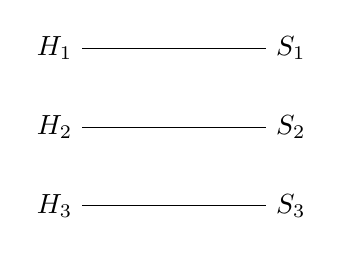
\begin{tikzpicture}[black/.style={circle,draw,fill=black,inner sep=0pt, minimum width=4pt}]
\node at (1,2) (1) {$H_1$};
\node at (1,1) (2) {$H_2$};
\node at (1,0) (3) {$H_3$};
\node at (4,2) (A) {$S_1$};
\node at (4,1) (B) {$S_2$};
\node at (4,0) (C) {$S_3$};
\draw (1) -- (A);
\draw (2) -- (B);
\draw (3) -- (C);
\end{tikzpicture}
\end{figure}
$(H_1, S_1)$, $(H_2, S_2)$, $(H_3, S_3)$:
\begin{figure}[H]
\centering
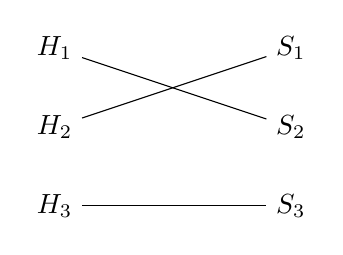
\begin{tikzpicture}[black/.style={circle,draw,fill=black,inner sep=0pt, minimum width=4pt}]
\node at (1,2) (1) {$H_1$};
\node at (1,1) (2) {$H_2$};
\node at (1,0) (3) {$H_3$};
\node at (4,2) (A) {$S_1$};
\node at (4,1) (B) {$S_2$};
\node at (4,0) (C) {$S_3$};
\draw (1) -- (B);
\draw (2) -- (A);
\draw (3) -- (C);
\end{tikzpicture}
\end{figure}


\subsection{} % Section 1.b
The Gale-Shapely algorithm -- in which hospitals propose to the students -- the output is $(H_1, S_1)$, $(H_2, S_2)$, $(H_3, S_3)$:
\begin{figure}[H]
\centering
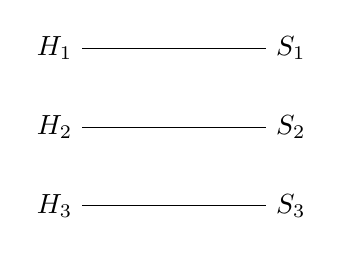
\begin{tikzpicture}[black/.style={circle,draw,fill=black,inner sep=0pt, minimum width=4pt}]
\node at (1,2) (1) {$H_1$};
\node at (1,1) (2) {$H_2$};
\node at (1,0) (3) {$H_3$};
\node at (4,2) (A) {$S_1$};
\node at (4,1) (B) {$S_2$};
\node at (4,0) (C) {$S_3$};
\draw (1) -- (A);
\draw (2) -- (B);
\draw (3) -- (C);
\end{tikzpicture}
\end{figure}


\section{} % Section 2
\subsection{} % Section 2.a
Consider the following set of intervals:
$(1,2)$, $(2,5)$, $(1,3)$, $(3,4)$.
\newline
\newline
The ``earliest finish time'' algorithm would allocate a first machine for $(1,2)$, and a second machine for $(1,3)$.
It would send $(3,4)$ to the first machine, since $(1,2)$ is now done, and finally it would allocate a third machine for $(2,5)$, since the first and second machines are already in use.
This interval is partitioned using only two machines using the ``earliest start time'' algorithm, and so the ``earliest finish time'' algorithm is not optimal.


\subsection{} % Section 2.b
We first observe that we need at least as many machines as we have jobs overlapping at any one point in time so the maximum number of mutually overlapping jobs is a lower bound for the number of machines we must use.

In the greedy algorithm, we check to see if any of the already allocated machines is compatible with each job before we give that job to the machine.
The only time we allocate a new machine is when this is not the case -- that is, every machine allocated so far is not compatible with the job.
This can only happen if there are already jobs running on every allocated machine
Since we sorted the jobs by start time, each of the running jobs started before the job we're currently trying to allocate, so we could not have allocated them any differently to use fewer machines.

The number of machines we allocate is therefore equal to the maximum number of mutually overlapping jobs -- our lower bound -- and thus the algorithm is optimal.


\section{} % Section 3
Suppose we came up with a way to multiply two $3\times3$ matrices using exactly 21 multiplications.
Our recurrence would look like
\[T(n) = 21T\left(\frac{n}{3}\right)+\Theta\left(n^2\right).\]
By the master theorem, since $2 < \log_321$, we have
\[T(n) \in \Theta\left(n^{\log_321}\right),\]
and $\log_321 < 2.807$, so this is indeed an improvement over Strassen's algorithm.


\section{} % Section 4
Below is our table after we've filled it out:
\begin{center}
\renewcommand{\arraystretch}{1.6}
\begin{tabular}{| c |c |c |c |c |c |c | c |}
	\hline
	  &   & P & A & L & A & T & E \\ \hline
	  & 0 & 2 & 4 & 6 & 8 & 10 & 12 \\ \hline
	P & 2 & 0 & 2 & 4 & 6 & 8 & 10 \\ \hline
	A & 4 & 2 & 0 & 2 & 4 & 6 & 8 \\ \hline
	L & 6 & 4 & 2 & 0 & 2 & 4 & 6 \\ \hline
	E & 8 & 6 & 4 & 2 & 1 & 3 & 5 \\ \hline
	T & 10 & 8 & 6 & 4 & 3 & 1 & 3 \\ \hline
	T & 12 & 10 & 8 & 6 & 5 & 3 & 2 \\ \hline
	E & 14 & 12 & 10 & 8 & 7 & 5 & 3 \\ \hline
\end{tabular}
\end{center}
Our final answer is 3, and it is obtained with the following alignment:
\newline
P A L A T -- E
\newline
P A L E T T E


\end{document}
